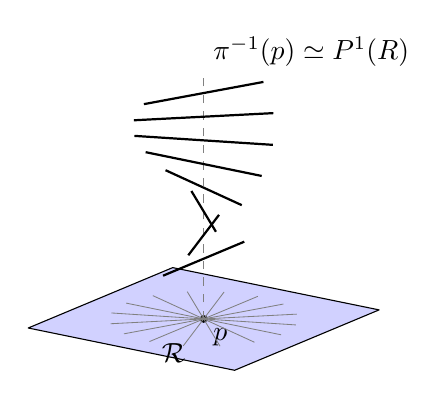
\begin{tikzpicture}[line join=round]
\filldraw[draw=black, line width=0.4pt, fill=blue!18] (-0.393,0.652) -- (-2.228,-0.115) -- (0.393,-0.652) -- (2.228,0.115) -- cycle;
\fill (0.000,0.000) circle (1.4pt);
\node[below right] at (0.000,0.000) {$p$};
\draw[gray, dashed] (0.000,0.000) -- (0.000,3.156);
\draw[thick] (0.516,0.981) -- (-0.516,0.549);
\draw[gray, line width=0.3pt] (0.688,0.287) -- (-0.688,-0.287);
\draw[thick] (0.195,1.322) -- (-0.195,0.809);
\draw[gray, line width=0.3pt] (0.260,0.343) -- (-0.260,-0.343);
\draw[thick] (-0.156,1.625) -- (0.156,1.107);
\draw[gray, line width=0.3pt] (-0.208,0.346) -- (0.208,-0.346);
\draw[thick] (-0.484,1.889) -- (0.484,1.445);
\draw[gray, line width=0.3pt] (-0.645,0.296) -- (0.645,-0.296);
\draw[thick] (-0.737,2.118) -- (0.737,1.816);
\draw[gray, line width=0.3pt] (-0.983,0.201) -- (0.983,-0.201);
\draw[thick] (-0.879,2.325) -- (0.879,2.211);
\draw[gray, line width=0.3pt] (-1.172,0.076) -- (1.172,-0.076);
\draw[thick] (-0.886,2.523) -- (0.886,2.614);
\draw[gray, line width=0.3pt] (-1.182,-0.061) -- (1.182,0.061);
\draw[thick] (-0.759,2.728) -- (0.759,3.010);
\draw[gray, line width=0.3pt] (-1.012,-0.189) -- (1.012,0.189);
\node[right] at (0.000,3.395) {$\pi^{-1}(p)\simeq\mathbb{P}^1(\mathbb{R})$};
\node[right] at (-0.656,-0.437) {$\mathcal{R}$};
\end{tikzpicture}
